\section{Rhythmic Similarity}\label{rhythmsimc}

This chapter provides an overview of some of the possibilities for computing music similarity by focusing on rhythmic features of different songs. \\
Nearly every MIR toolkit provides an extraction tool for the beats per minute (BPM) and thus the tempo of each song. The most trivial solution of computing very low-level rhythmic similarities is by sorting and comparing songs only by their main tempo (BPM). There are certainly far better and more accurate solutions.
%By just comparing the tempo of songs, a lot of rhythm information is lost, e.g., the rhythmic structures of songs like the time signature, up- and downbeats, etc.\\ 
This chapter presents some of the most promising approaches to compute rhythm similarities regarding the applicability in a Big Data framework.\\

\subsection{Beat Histogram}\label{beathist}

One possible similarity measurement is, e.g., the usage of beat histograms as proposed by Tsanetakis and Cook~\cite{rhythm3}. The Essentia toolkit offers methods to extract the beat histogram. The different detected BPMs are normalized to 1. If a song changes its tempo, then multiple peaks can be seen.
\begin{figure}[htbp]
	\centering
	\framebox{\parbox{1\textwidth}{
			\begin{subfigure}{.495\textwidth}
				\centering
				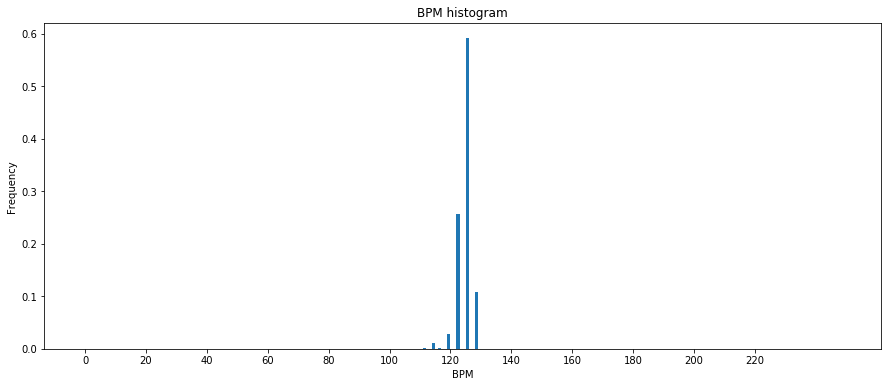
\includegraphics[scale=0.25]{Images/Beat/h_o_bh.png}
				\caption{Rock You Like A Hurricane, Scorpions}
				\label{hobh}
			\end{subfigure}%
			\begin{subfigure}{.495\textwidth}
				\centering
				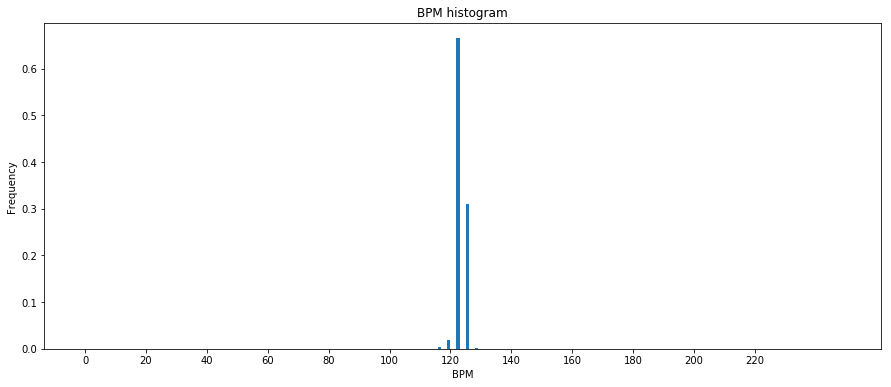
\includegraphics[scale=0.25]{Images/Beat/h_c_bh.png}
				\caption{Rock You Like A Hurricane, Knightsbridge}
				\label{hcbh}
			\end{subfigure}% 
			
			\begin{subfigure}{.495\textwidth}
				\centering
				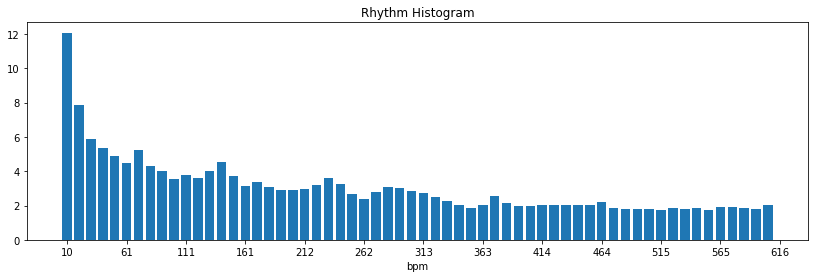
\includegraphics[scale=0.25]{Images/Beat/s_s_bh.png}
				\caption{Behind Space, 94' version}
				\label{ssbh}
			\end{subfigure}%
			\begin{subfigure}{.495\textwidth}
				\centering
				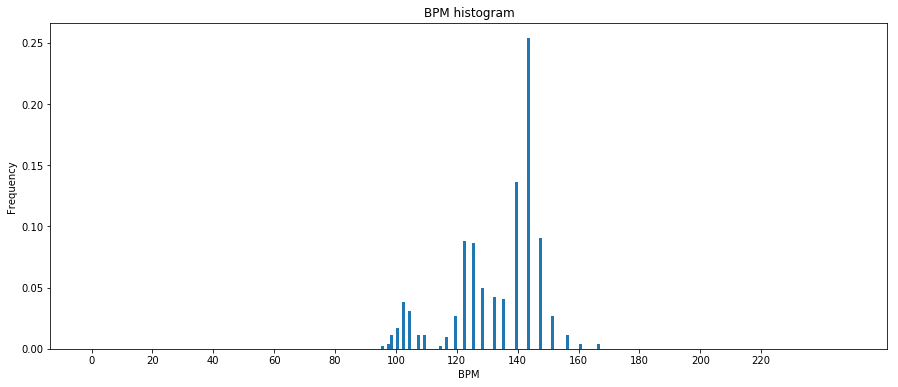
\includegraphics[scale=0.25]{Images/Beat/s_a_bh.png}
				\caption{Behind Space, 99' version}
				\label{sabh}
			\end{subfigure}%			
	}}
	\caption{Beat histogram examples}
	\label{fig:bh1}
\end{figure}
\noindent Figure~\ref{fig:bh1} shows the beat histograms of the song "Rock you like a hurricane" by the Scorpions (Figure \ref{hobh}) and covered by Knightsbridge(Figure \ref{hcbh}) as well as two different versions of the song "Behind Space" from the Swedish metal band In Flames, one is sung by Stanne Mikkels in 1994 (Figure \ref{ssbh}) and the second version was recorded with Anders Friden as the vocalist in 1999 (Figure \ref{sabh}). The 1994 version changes its tempo in the outro of the song, and the tempo change can be seen in the histogram in Figure~\ref{ssbh} as a second large peak around 120 BPM.
Similarities between two beat histograms can be computed using the Euclidean distance. 
\noindent Gruhne (et al.) further improved beat histograms and suggested an additional post-processing step before calculating the similarity between songs with the Euclidean distance. They found that logarithmic re-sampling of the lag axis of the histogram and cross-correlation with an artificial rhythmic grid improves the performance of this similarity measurement further (see~\cite[182]{rbh1}). This thesis does not use the additional re-sampling.\\
\noindent Another paper that is just mentioned here (one of the older ones from 2002) uses the beat spectrum as a feature~\cite{rhythm1} to compute similarities.

\subsection{Rhythm Patterns}\label{flucpat}

A more state-of-the-art feature is the so-called rhythm pattern, also known as fluctuation patterns, evaluated by Lidy and Rauber in~\cite{rp1} for instance. 
To extract these features, the rp\_extractor library for Python~\cite{rp_extract} was made publicly available by the TU Vienna~\cite{rp_extract2}. Figure~\ref{fig:rp1} shows the extracted rhythmic patterns of the previously mentioned songs "Rock you like a Hurricane" and "Behind Space". The similarities of the different versions from the same songs are quite visible, while at the same time substantial differences between the different songs are recognizable.

\begin{figure}[htbp]
	\centering
	\framebox{\parbox{1\textwidth}{
			\begin{subfigure}{.495\textwidth}
				\centering
				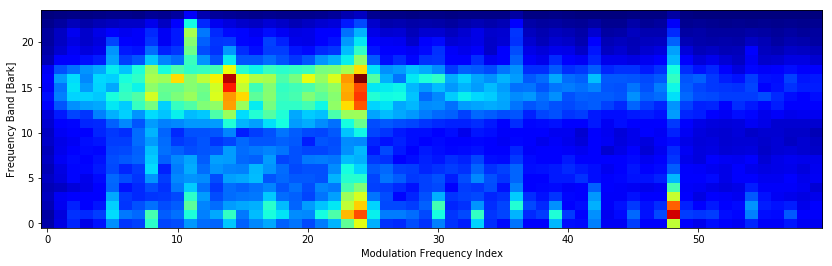
\includegraphics[scale=0.25]{Images/Beat/h_o_rp.png}
				\caption{Rock You Like A Hurricane, Scorpions}
				\label{horp}
			\end{subfigure}%
			\begin{subfigure}{.495\textwidth}
				\centering
				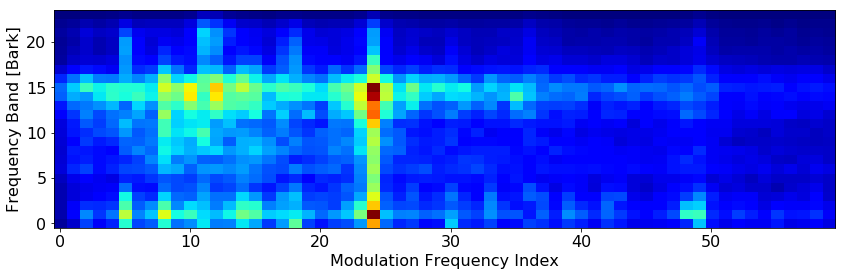
\includegraphics[scale=0.25]{Images/Beat/h_c_rp.png}
				\caption{Rock You Like A Hurricane, Knightsbridge}
				\label{hcrp}
			\end{subfigure}% 
			
			\begin{subfigure}{.495\textwidth}
				\centering
				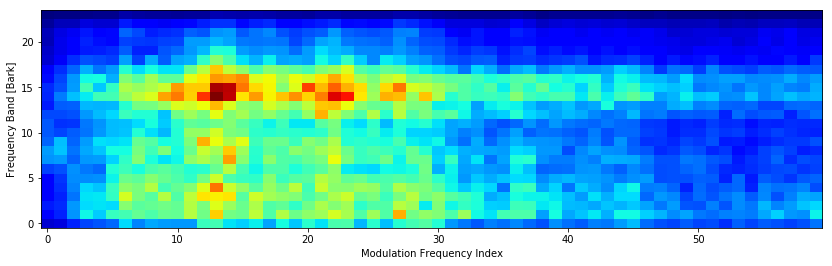
\includegraphics[scale=0.25]{Images/Beat/s_s_rp.png}
				\caption{Behind Space, 94' version}
				\label{ssrp}
			\end{subfigure}%
			\begin{subfigure}{.495\textwidth}
				\centering
				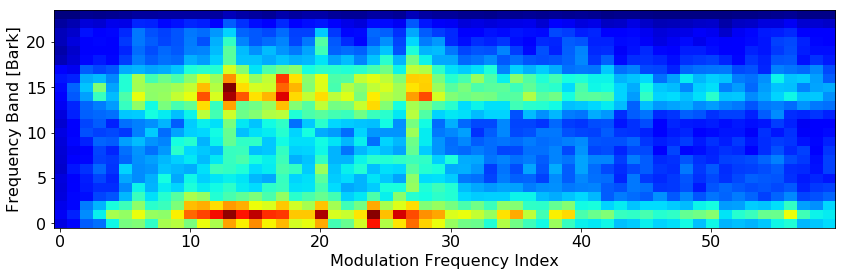
\includegraphics[scale=0.25]{Images/Beat/s_a_rp.png}
				\caption{Behind Space, 99' version}
				\label{sarp}
			\end{subfigure}%			
	}}
	\caption{Rhythm pattern examples}
	\label{fig:rp1}
\end{figure}

\noindent The x-axis represents the frequency bands converted to the Bark-scale (a scale representing the human auditory system comparable to the mel scale from Equation~\eqref{eq:mel}), and the y-axis represents the modulation frequency index representing the modulation frequencies up to 10Hz (around 600 BPM).
The Bark of a frequency $f$ can be determined using the equation
\begin{equation} \label{eq:bark}
\text{Bark} = 13 \arctan(0.00076 f) + 3.5 \arctan ((f / 7500)^2).
\end{equation}
The algorithm to extract rhythm patterns, rhythm histogram, and statistical spectrum descriptors measuring the variations over the critical frequency bands, can be seen in Figure~\ref{fig:rpe}.

\begin{center}
  % setting the typeface to sans serif and the font size to small
  % the scope local to the environment
  \sffamily
  \footnotesize
  \begin{tikzpicture}[auto,
    %decision/.style={diamond, draw=black, thick, fill=white,
    %text width=8em, text badly centered,
    %inner sep=1pt, font=\sffamily\small},
    block_center/.style ={rectangle, draw=black, thick, fill=white,
      text width=16em, text centered,
      minimum height=2em},
    block_left/.style ={rectangle, draw=black, thick, fill=white,
      text width=16em, text ragged, minimum height=2em, inner sep=6pt},
    block_noborder/.style ={rectangle, draw=none, thick, fill=none,
      text width=18em, text centered, minimum height=1em},
    block_assign/.style ={rectangle, draw=black, thick, fill=white,
      text width=18em, text ragged, minimum height=2em, inner sep=6pt},
    block_lost/.style ={rectangle, draw=black, thick, fill=white,
      text width=16em, text ragged, minimum height=2em, inner sep=6pt},
      line/.style ={draw, thick, -latex', shorten >=0pt}]
    % outlining the flowchart using the PGF/TikZ matrix funtion
    \matrix [column sep=5mm,row sep=3mm] {
      % enrollment - row 1
      \node [block_center] (audiosig) {Audio Signal};\\
      % enrollment - row 2
      \node [block_center] (pre) {Pre-Processing};\\
      % enrollment - row 3
      \node [block_center] (stft) {Power Spectrum (STFT)};\\ 
      % follow-up - row 4
      \node [block_center] (bark) {Critical Bands (Bark scale)};\\
      % follow-up - row 5
      \node [block_center] (phon) {Equal Loudness (Phon)};\\
      % follow-up - row 6
      \node [block_center] (sone) {Specific Loudness Sens. (Sone)};
	  & \node [block_assign] (stat) {Statistical Spectrum Descriptor $\rightarrow$ \textit{\textbf{SSD}}};\\
      % follow-up - row 7
	  \node [block_center] (fft) {Modulation Amplitude (FFT)};
 	  & \node [block_assign] (rh) {Rhythm Histogram $\rightarrow$ \textit{\textbf{RH}}};\\
       % follow-up - row 8
      \node [block_center] (fsw) {Fluctuation Strength Weighting};\\
      % follow-up - row 9
      \node [block_center] (filt) {Filtering / Blurring};
   	  & \node [block_assign] (rp) {Rhythmic Patterns $\rightarrow$ \textit{\textbf{RP}}};\\
    };% end matrix
    % connecting nodes with paths
    \begin{scope}[every path/.style=line]
      % paths for enrollemnt rows
      \path (audiosig)   -- (pre);
      \path (pre)  -- (stft);
      \path (stft) -- (bark);
      \path (bark) -- (phon);
      \path (phon) -- (sone);
      \path (sone) -- (stat);
      \path (sone) -- (fft);
      \path (fft) -- (rh);
      \path (fft) -- (fsw);
      \path (fsw) -- (filt);
      \path (filt) -- (rp);
    \end{scope}
  \end{tikzpicture}
  	\captionof{figure}{Rhythm pattern extraction procedure as suggested by~\cite{rp_extract2}}
	\label{fig:rpe}
\end{center}

\noindent In conclusion, the rhythm patterns basically represent the BPM of various frequency bands.
To compare two different songs the Euclidean distance between the vectorized rhythm pattern matrices can be calculated as Pampalk suggests~\cite[p. 40]{fp1}.\\
Pohle, Schnitzer (et al.)~\cite{rp2} later refined fluctuation patterns into onset patterns, e.g., by using semitone bands instead of fewer critical bands to detect onsets. This thesis however, focuses on fluctuation-/ rhythm patterns extracted with the rp\_extractor library. 

\subsection{Rhythm Histogram}

A more simplistic and lower-dimensional feature coming with the rp\_extract toolkit is the rhythm histogram. "The Rhythm Histogram features we use are a descriptor for general rhythmics in an audio document. Contrary to the Rhythm Patterns and the Statistical Spectrum Descriptor, information is not stored per critical band. Rather, the magnitudes of each modulation frequency bin of all 24 critical bands are summed up, to form a histogram of "rhythmic energy" per modulation frequency. The histogram contains 60 bins which reflect modulation frequency between 0 and 10 Hz."~\cite[p. 3]{rp1}. 
The difference between rhythm histogram and the earlier in Section~\ref{beathist} mentioned beat histogram appears to be the beat histogram focusing on the basic tempo of the whole song while the rhythm histogram takes all frequency bands and therefore the sub-rhythms of single instruments into account. Figure \ref{fig:rh1} shows the rhythm histograms of four example songs. 

\begin{figure}[htbp]
	\centering
	\framebox{\parbox{1\textwidth}{
			\begin{subfigure}{.495\textwidth}
				\centering
				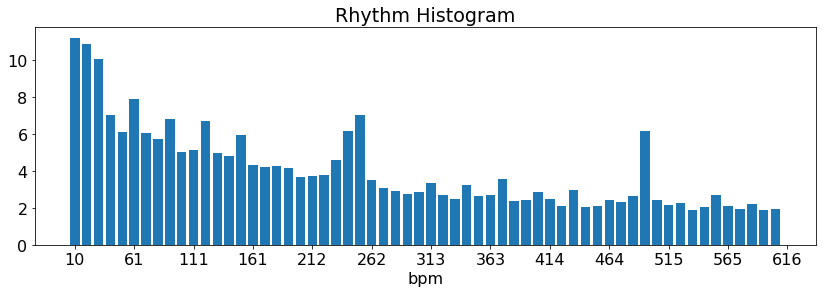
\includegraphics[scale=0.25]{Images/Beat/h_o_rh.png}
				\caption{Rock You Like A Hurricane, Scorpions}
				\label{horh}
			\end{subfigure}%
			\begin{subfigure}{.495\textwidth}
				\centering
				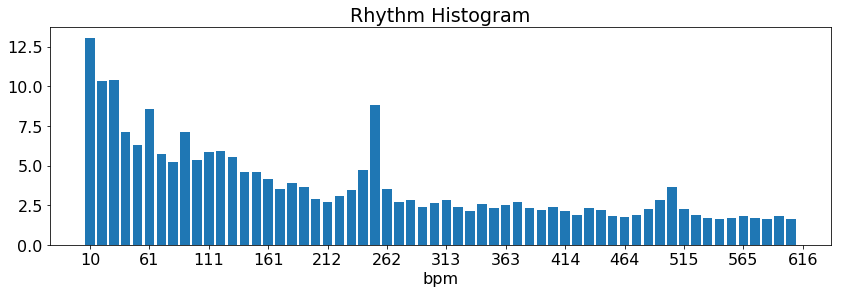
\includegraphics[scale=0.25]{Images/Beat/h_c_rh.png}
				\caption{Rock You Like A Hurricane, Knightsbridge}
				\label{hcrh}
			\end{subfigure}% 
			
			\begin{subfigure}{.495\textwidth}
				\centering
				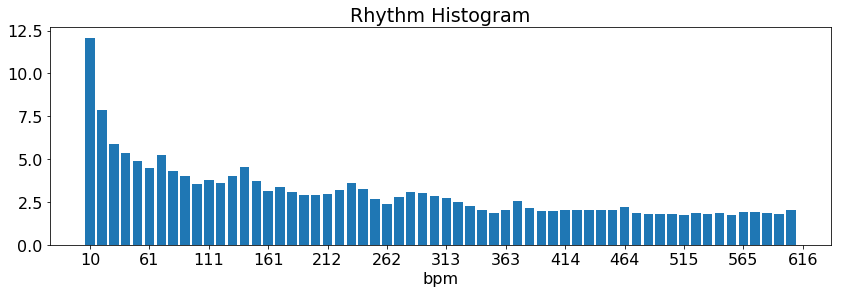
\includegraphics[scale=0.25]{Images/Beat/s_s_rh.png}
				\caption{Behind Space, 94' version}
				\label{ssrh}
			\end{subfigure}%
			\begin{subfigure}{.495\textwidth}
				\centering
				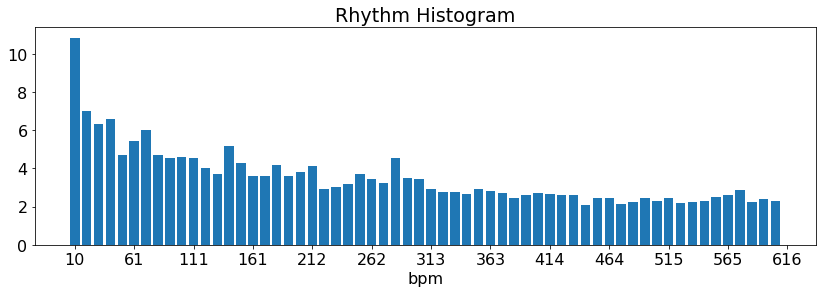
\includegraphics[scale=0.25]{Images/Beat/s_a_rh.png}
				\caption{Behind Space, 99' version}
				\label{sarh}
			\end{subfigure}%			
	}}
	\caption{Rhythm histogram examples}
	\label{fig:rh1}
\end{figure}

\subsection{Cross-Correlation}

Estimating the onset strength as introduced in section \ref{otheraudiofeat}, averaging it per beat and creating a discrete-time signal for each song is another possibility. Similar to the chroma features, the cross-correlation of these discrete-time onset features could be used as a similarity measurement, following Equation \ref{eq:conv1}. 

\begin{figure}[htbp]
	\centering
	\framebox{\parbox{1\textwidth}{ 			
			\begin{subfigure}{.495\textwidth}
				\centering    
				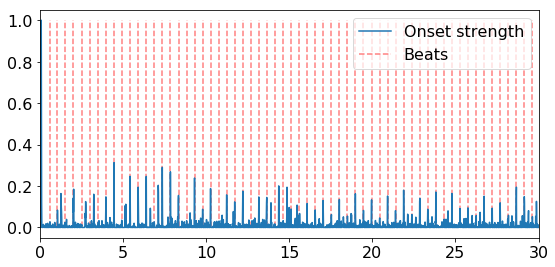
\includegraphics[scale=0.3]{Images/Beat/h_o_on.png}
				\caption{Rock You Like A Hurricane, Scorpions}
				\label{hoon}
			\end{subfigure}		
			\begin{subfigure}{.495\textwidth}
				\centering     
				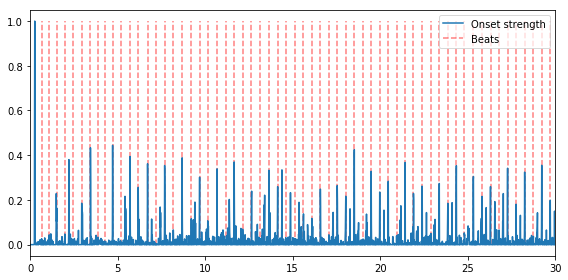
\includegraphics[scale=0.3]{Images/Beat/h_c_on.png}
				\caption{Rock You Like A Hurricane, Knightsbridge}
				\label{hcon}
			\end{subfigure}%	
				
			\begin{subfigure}{.495\textwidth}
				\centering    
				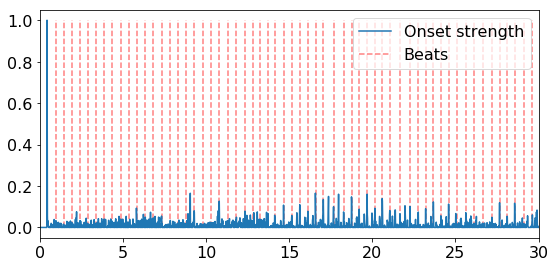
\includegraphics[scale=0.3]{Images/Beat/s_s_on.png}
				\caption{Behind Space, 94' version}
				\label{saon}
			\end{subfigure}		
			\begin{subfigure}{.495\textwidth}
				\centering     
				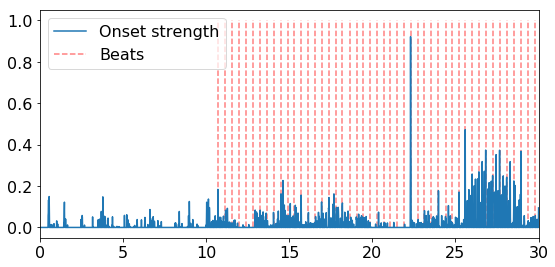
\includegraphics[scale=0.3]{Images/Beat/s_a_on.png}
				\caption{Behind Space, 99' version}
				\label{sson}
			\end{subfigure}%			
				
	}}
	\caption{Detected onset examples (30 second song snippets)}
	\label{fig:ons1}
\end{figure}	

\noindent Looking at the extracted onset features of the Song "Behind Space" by In Flames (sung by Anders Frieden 99' and Stanne Mikkels 94') in Figure~\ref{fig:ons1}, one can see that the quality of these signals is greatly dependent on the underlying beat extraction and onset detection algorithms. As an example, the librosa toolkit struggles to detect beats in the first 10 seconds of the song "Behind Space" recorded in 1999. Also, this representation seems to contain a lot less valuable and comparable information in contrast to fluctuation patterns. In conclusion, this approach is discarded and not further considered and tested in this thesis.  

\section{Summary}\label{sumfeat}

After evaluating various options of similarity measurements for different aspects of music (timbre, rhythm, and melody), all of the chosen approaches that are implemented in the next chapters are summarized in this section.\\
The chosen similarity metrics for timbre similarity are: 
\begin{itemize}
	\setlength\itemsep{-0.5em}
	\item Euclidean Distance
	\item symmetric Kullback-Leibler divergence
	\item Jensen-Shannon-like divergence
\end{itemize}
For the computation of the melodic similarities, two different similarity metrics are chosen: 
\begin{itemize}
	\setlength\itemsep{-0.5em}
	\item Levenshtein Distance 
	\item cross-correlation on full beat aligned and per beat averaged chroma features, key shifted to A
\end{itemize}
Three different similarity measurements are chosen for the rhythm features: 
\begin{itemize}
	\setlength\itemsep{-0.5em}
	\item Euclidean distance between beat histograms
	\item Euclidean distance between rhythm histograms
	\item Euclidean distance between rhythm patterns
\end{itemize}



